\documentclass[conference]{IEEEtran}
\IEEEoverridecommandlockouts

% Packages
\usepackage{cite}
\usepackage{amsmath,amssymb,amsfonts}
\usepackage{algorithmic}
\usepackage{graphicx}
\usepackage{textcomp}
\usepackage{xcolor}
\usepackage{tikz}
\usepackage{pgfplots}
\usepackage{booktabs}
\usepackage{multirow}
\usepackage{listings}
\usepackage{url}
\usepackage{hyperref}
\usepackage{float}

\pgfplotsset{compat=1.17}
\usetikzlibrary{shapes,arrows,positioning,fit,backgrounds,calc,decorations.pathreplacing}

% Code listing style
\lstdefinestyle{spice}{
    basicstyle=\ttfamily\scriptsize,
    breaklines=true,
    frame=single,
    numbers=left,
    numberstyle=\tiny,
    keywordstyle=\color{blue},
    commentstyle=\color{green!60!black},
    stringstyle=\color{red},
}

\lstdefinestyle{python}{
    basicstyle=\ttfamily\scriptsize,
    breaklines=true,
    frame=single,
    numbers=left,
    numberstyle=\tiny,
    keywordstyle=\color{blue},
    commentstyle=\color{green!60!black},
    stringstyle=\color{orange},
    language=Python,
}

\def\BibTeX{{\rm B\kern-.05em{\sc i\kern-.025em b}\kern-.08em
    T\kern-.1667em\lower.7ex\hbox{E}\kern-.125emX}}

\begin{document}

\title{ModelIR: A Semantic Translation Framework for Cross-Simulator SPICE Device Models with Automated Verification}

\author{\IEEEauthorblockN{Author Name}
\IEEEauthorblockA{\textit{Department of Electrical Engineering} \\
\textit{University Name}\\
City, Country \\
email@university.edu}
}

\maketitle

\begin{abstract}
Modern integrated circuit design flows increasingly require interoperability between multiple SPICE simulators, yet foundry-provided device models are typically locked to a single simulator format. This paper presents ModelIR, an open-source semantic translation framework that enables automatic conversion of device model libraries between Spectre, HSPICE, and ngspice formats. Unlike simple syntactic translators, ModelIR employs a canonical intermediate representation that captures device physics semantics, enabling correct handling of format-specific constructs such as capacitor parasitic models, BSIM level mappings, and temperature coefficient translations. The framework implements a three-phase compiler architecture consisting of format-specific parsers, a device-agnostic intermediate representation layer, and target-specific code generators with semantic lowering capabilities. We validate ModelIR on a comprehensive corpus of 82 production PDK files from seven foundries and academic sources, successfully translating 699 device models with 100\% ngspice syntax verification pass rate. Electrical verification through DC operating point and I-V characteristic analysis confirms functional equivalence of translated models. Performance benchmarks demonstrate translation throughput of 118 models per second, reducing PDK porting effort from weeks of manual work to seconds of automated translation.
\end{abstract}

\begin{IEEEkeywords}
SPICE simulation, device models, PDK translation, BSIM, intermediate representation, compiler architecture, EDA tools
\end{IEEEkeywords}

%==============================================================================
\section{Introduction}
%==============================================================================

The semiconductor industry relies extensively on SPICE simulation for circuit verification throughout the design process, from initial concept exploration through final signoff. However, different organizations have standardized on different simulation platforms based on historical factors, licensing arrangements, and specific technical requirements. Commercial foundries typically provide Process Design Kits optimized for Synopsys HSPICE or Cadence Spectre, while academic institutions and emerging companies increasingly adopt open-source alternatives such as ngspice for reasons of cost, accessibility, and customization flexibility.

This fragmentation of the SPICE ecosystem creates a significant practical barrier for design teams. Engineers cannot freely choose their simulation tool without undertaking substantial manual effort to port device model libraries from one format to another. A typical advanced-node PDK contains hundreds of device models encompassing MOSFETs, bipolar transistors, diodes, resistors, and capacitors, with each model specified by thousands of parameters that must be correctly translated. Manual translation of such libraries is not only time-consuming but also highly error-prone, as subtle syntactic differences between simulators can result in incorrect electrical behavior that may not be immediately apparent.

Previous approaches to SPICE interoperability have focused primarily on netlist conversion, treating device models as opaque references that need not be modified. While this approach enables schematic-level translation, it does not address the fundamental problem of model library portability. The device models themselves, containing BSIM compact model parameters, parasitic subcircuit definitions, and simulator-specific syntax extensions, remain locked to their original format.

This paper addresses the model library translation problem through a systematic compiler-based approach. The key insight is that while SPICE dialects differ significantly in syntax, they share a common underlying semantic model rooted in device physics. By capturing this semantic content in a canonical intermediate representation, translation becomes a matter of format-specific parsing and generation rather than ad-hoc pattern matching.

The remainder of this paper is organized as follows. Section II provides background on SPICE simulator differences and reviews related work in EDA tool interoperability. Section III presents the detailed system architecture of ModelIR, including the intermediate representation design and semantic lowering strategies. Section IV describes the implementation of key components. Section V presents comprehensive evaluation results including corpus translation statistics, electrical verification, and performance benchmarks. Section VI discusses limitations and future directions, and Section VII concludes.

%==============================================================================
\section{Background and Related Work}
%==============================================================================

\subsection{SPICE Simulator Ecosystem}

The three major SPICE dialects targeted by ModelIR represent distinct evolutionary paths from the original Berkeley SPICE3 codebase. Table~\ref{tab:simulators} summarizes the key differences between these simulators that must be handled during translation.

\begin{table}[htbp]
\caption{Comparison of Target SPICE Simulators}
\label{tab:simulators}
\centering
\begin{tabular}{p{2.2cm}ccc}
\toprule
\textbf{Feature} & \textbf{Spectre} & \textbf{HSPICE} & \textbf{ngspice} \\
\midrule
Vendor & Cadence & Synopsys & Open-source \\
License cost & \$100K+ & \$80K+ & Free \\
Model syntax & \texttt{model n nmos} & \texttt{.model n nmos} & \texttt{.model n nmos} \\
Include directive & \texttt{include} & \texttt{.include} & \texttt{.include} \\
Section selection & \texttt{section=xx} & \texttt{.lib 'f' xx} & \texttt{.lib 'f' xx} \\
BSIM4 level & 14 & 54 & 14 or 54 \\
Case sensitivity & Yes & No & No \\
Line continuation & \texttt{\textbackslash} & \texttt{+} & \texttt{+} \\
\bottomrule
\end{tabular}
\end{table}

Cadence Spectre originated as a native simulator for the Virtuoso design environment and employs a syntax that differs substantially from traditional SPICE. Model definitions omit the leading dot, use different keywords for subcircuit boundaries, and support inline parameter expressions that are evaluated during parsing rather than simulation. Spectre is case-sensitive, meaning that parameter names must match exactly between model definitions and instantiations.

Synopsys HSPICE evolved from commercial enhancements to Berkeley SPICE and maintains closer syntactic compatibility with the original format while adding numerous proprietary extensions. HSPICE uses a different set of level numbers for BSIM models, employs its own library sectioning mechanism, and supports optimization and Monte Carlo features not available in the original SPICE.

The ngspice project represents the open-source continuation of Berkeley SPICE3f5, with ongoing development adding modern features while maintaining backward compatibility. ngspice can accept either HSPICE-style or traditional SPICE level numbers for most models, though some advanced features require specific syntax adaptations.

\subsection{BSIM Compact Model Family}

The Berkeley Short-channel IGFET Model family represents the industry standard for MOSFET compact modeling across technology nodes from 0.5$\mu$m down to sub-10nm FinFET processes. Different BSIM versions use different level numbers to identify the model equations, and these level numbers vary between simulators as shown in Table~\ref{tab:levels}.

\begin{table}[htbp]
\caption{BSIM Level Number Mappings Across Simulators}
\label{tab:levels}
\centering
\begin{tabular}{lccc}
\toprule
\textbf{Model Version} & \textbf{HSPICE} & \textbf{ngspice} & \textbf{Spectre} \\
\midrule
BSIM3v3 & 49 & 8, 49 & 11 \\
BSIM4.0--4.5 & 54 & 14, 54 & 14 \\
BSIM4.6--4.8 & 54 & 14 & 14 \\
BSIM-SOI & 57 & 10 & --- \\
BSIM-CMG (FinFET) & 72 & OSDI & 16 \\
EKV & 55 & 55 & --- \\
\bottomrule
\end{tabular}
\end{table}

A significant challenge in model translation is that the same physical model equations are identified by different level numbers depending on the simulator. A naive text-based translation that preserves level numbers verbatim will produce incorrect simulations when the target simulator interprets that level as a different model type.

\subsection{Related Work}

Several commercial and academic efforts have addressed aspects of SPICE interoperability, though none provide the comprehensive model library translation capability of ModelIR.

Commercial netlist translators integrated into design environments such as Cadence Virtuoso and Synopsys Custom Compiler can convert schematic-level netlists between formats. However, these tools treat device models as opaque references, requiring that compatible model libraries already exist in the target format. The burden of model translation remains with the user.

Foundry PDK porting tools provided by some semiconductor manufacturers enable one-way conversion, typically from Spectre to HSPICE. These tools are proprietary, foundry-specific, and generally available only under NDA as part of PDK licensing agreements. They do not support translation to open-source simulators.

The OpenPDK initiatives led by Google and partner foundries have produced fully open-source PDKs for processes including SkyWater 130nm and GlobalFoundries 180nm. While these PDKs provide models in multiple formats, they represent parallel development efforts rather than automated translation, and the approach does not scale to proprietary PDKs.

Academic work on SPICE interoperability has focused primarily on model equation verification and behavioral equivalence checking. These approaches validate that models produce correct simulation results but do not address the syntactic translation problem.

To the authors' knowledge, ModelIR is the first open-source tool that performs semantic translation of complete device model libraries across multiple SPICE dialects while preserving electrical correctness.

%==============================================================================
\section{System Architecture}
%==============================================================================

ModelIR implements a classic three-phase compiler architecture adapted for the domain of SPICE device model translation. This section describes the overall system structure, the design of the intermediate representation, and the semantic lowering strategies that enable correct translation of format-specific constructs.

\subsection{Architectural Overview}

The high-level architecture of ModelIR follows the established compiler pattern of separating source language parsing from target language generation through an intermediate representation. Fig.~\ref{fig:architecture} illustrates the complete translation pipeline.

\begin{figure}[htbp]
\centering
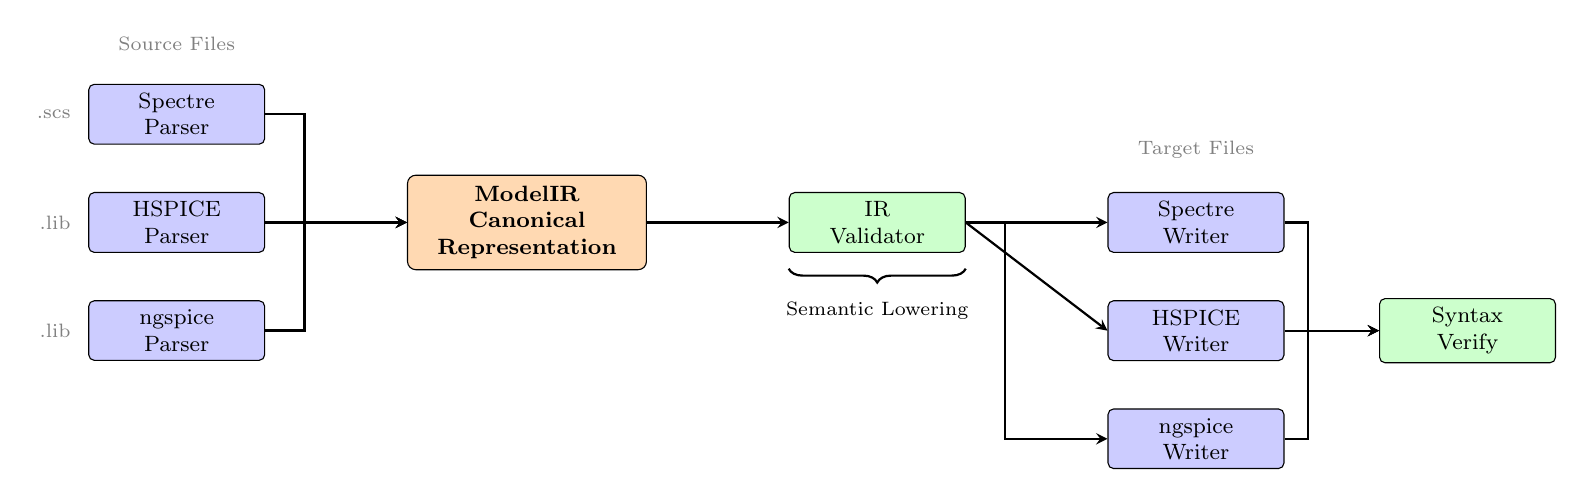
\begin{tikzpicture}[
    node distance=0.6cm and 1.2cm,
    block/.style={rectangle, draw, fill=blue!20, text width=2cm, text centered, minimum height=0.7cm, font=\footnotesize, rounded corners=2pt},
    ir/.style={rectangle, draw, fill=orange!30, text width=2.8cm, text centered, minimum height=1.2cm, font=\footnotesize\bfseries, rounded corners=3pt},
    valid/.style={rectangle, draw, fill=green!20, text width=2cm, text centered, minimum height=0.7cm, font=\footnotesize, rounded corners=2pt},
    arrow/.style={->, >=stealth, thick},
    label/.style={font=\scriptsize, text=gray}
]
    % Input files
    \node[label] (in_label) {Source Files};
    \node[block, below=0.3cm of in_label] (spectre) {Spectre\\Parser};
    \node[block, below=of spectre] (hspice) {HSPICE\\Parser};
    \node[block, below=of hspice] (ngspice_p) {ngspice\\Parser};
    
    % IR
    \node[ir, right=1.8cm of hspice] (ir) {ModelIR\\Canonical\\Representation};
    
    % Validation
    \node[valid, right=1.8cm of ir] (valid) {IR\\Validator};
    
    % Output writers
    \node[block, right=1.8cm of valid] (spectre_w) {Spectre\\Writer};
    \node[block, below=of spectre_w] (hspice_w) {HSPICE\\Writer};
    \node[block, below=of hspice_w] (ngspice_w) {ngspice\\Writer};
    
    % Verification
    \node[valid, right=1.2cm of hspice_w] (verify) {Syntax\\Verify};
    
    % Output label
    \node[label, above=0.3cm of spectre_w] (out_label) {Target Files};
    
    % Arrows from parsers to IR
    \draw[arrow] (spectre.east) -- ++(0.5,0) |- (ir.west);
    \draw[arrow] (hspice.east) -- (ir.west);
    \draw[arrow] (ngspice_p.east) -- ++(0.5,0) |- (ir.west);
    
    % Arrow from IR to validator
    \draw[arrow] (ir) -- (valid);
    
    % Arrows from validator to writers
    \draw[arrow] (valid.east) -- ++(0.5,0) |- (spectre_w.west);
    \draw[arrow] (valid.east) -- (hspice_w.west);
    \draw[arrow] (valid.east) -- ++(0.5,0) |- (ngspice_w.west);
    
    % Arrows to verification
    \draw[arrow] (spectre_w.east) -- ++(0.3,0) |- (verify.west);
    \draw[arrow] (hspice_w.east) -- (verify.west);
    \draw[arrow] (ngspice_w.east) -- ++(0.3,0) |- (verify.west);
    
    % File type labels
    \node[label, left=0.1cm of spectre] {.scs};
    \node[label, left=0.1cm of hspice] {.lib};
    \node[label, left=0.1cm of ngspice_p] {.lib};
    
    % Semantic lowering annotation
    \draw[decorate, decoration={brace, amplitude=5pt, mirror}, thick] 
        ([yshift=-0.2cm]valid.south west) -- ([yshift=-0.2cm]valid.south east)
        node[midway, below=0.3cm, font=\scriptsize] {Semantic Lowering};
\end{tikzpicture}
\caption{ModelIR three-phase translation architecture showing the complete pipeline from source file parsing through intermediate representation to target file generation with syntax verification.}
\label{fig:architecture}
\end{figure}

The translation process begins with format-specific parsing. Each supported SPICE dialect has a dedicated parser that understands its particular syntax, including variations in line continuation, comment styles, and keyword conventions. The parsers produce a common intermediate representation that captures the semantic content of the device models independent of syntactic details.

The intermediate representation serves as the central data structure of the system. It provides a canonical format for device models that abstracts away simulator-specific syntax while preserving all information necessary for correct electrical simulation. The IR includes explicit representations for device types, polarities, model parameters, and structural elements such as subcircuits.

Following IR construction, an optional validation phase checks the intermediate representation for semantic consistency. This validation catches errors such as missing required parameters, invalid level numbers, and malformed expressions before code generation begins.

The final phase generates output in the target format using format-specific writers. These writers implement semantic lowering, the process of translating high-level constructs in the IR to equivalent lower-level constructs in the target format when direct translation is not possible.

\subsection{Intermediate Representation Design}

The design of the intermediate representation reflects a careful balance between abstraction and fidelity. The IR must be abstract enough to serve as a common target for multiple source formats, yet detailed enough to enable correct regeneration in any target format.

Fig.~\ref{fig:ir_structure} illustrates the hierarchical structure of the ModelIR intermediate representation.

\begin{figure}[htbp]
\centering
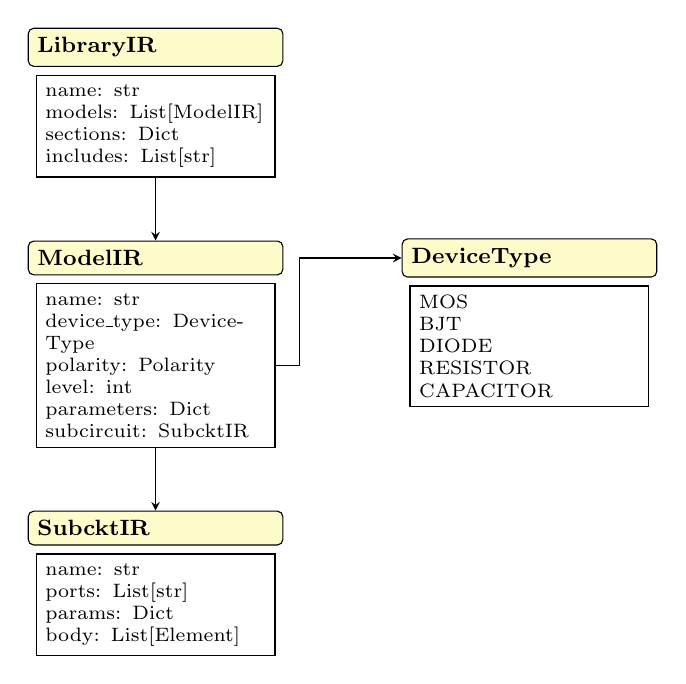
\begin{tikzpicture}[
    node distance=0.4cm,
    class/.style={rectangle, draw, fill=yellow!20, text width=3cm, font=\footnotesize, align=left, rounded corners=2pt},
    field/.style={rectangle, draw, fill=white, text width=2.8cm, font=\scriptsize, align=left},
    arrow/.style={->, >=stealth}
]
    % LibraryIR
    \node[class] (lib) {\textbf{LibraryIR}};
    \node[field, below=0.1cm of lib] (lib_f) {
        name: str\\
        models: List[ModelIR]\\
        sections: Dict\\
        includes: List[str]
    };
    
    % ModelIR
    \node[class, below=0.8cm of lib_f] (model) {\textbf{ModelIR}};
    \node[field, below=0.1cm of model] (model_f) {
        name: str\\
        device\_type: DeviceType\\
        polarity: Polarity\\
        level: int\\
        parameters: Dict\\
        subcircuit: SubcktIR
    };
    
    % DeviceType enum
    \node[class, right=1.5cm of model] (dtype) {\textbf{DeviceType}};
    \node[field, below=0.1cm of dtype] (dtype_f) {
        MOS\\
        BJT\\
        DIODE\\
        RESISTOR\\
        CAPACITOR
    };
    
    % SubcktIR
    \node[class, below=0.8cm of model_f] (sub) {\textbf{SubcktIR}};
    \node[field, below=0.1cm of sub] (sub_f) {
        name: str\\
        ports: List[str]\\
        params: Dict\\
        body: List[Element]
    };
    
    % Arrows
    \draw[arrow] (lib_f.south) -- (model.north);
    \draw[arrow] (model_f.east) -- ++(0.3,0) |- (dtype.west);
    \draw[arrow] (model_f.south) -- (sub.north);
    
\end{tikzpicture}
\caption{Hierarchical structure of the ModelIR intermediate representation showing the relationship between library, model, and subcircuit elements.}
\label{fig:ir_structure}
\end{figure}

At the top level, the LibraryIR class represents a complete model library file. It contains a list of ModelIR instances representing individual device models, along with metadata such as library sections for corner-specific model selection and include directives for external file references.

Each ModelIR instance encapsulates a single device model with all its defining characteristics. The device type field classifies the model as a MOSFET, BJT, diode, resistor, or capacitor, enabling type-specific handling during code generation. The polarity field distinguishes N-type from P-type devices for transistors. The level field contains the canonical BSIM level number, normalized to a common convention regardless of the source format.

The parameters dictionary contains all model parameters as name-value pairs. Parameter values may be numeric constants, expressions involving other parameters, or references to global variables. The IR preserves expression structure to enable correct evaluation in the target simulator.

For complex devices that require parasitic modeling, the optional subcircuit field contains a SubcktIR instance representing an equivalent circuit. This structure enables semantic lowering of high-level device specifications to equivalent subcircuit implementations.

\subsection{Semantic Lowering Strategies}

A key innovation in ModelIR is the concept of semantic lowering, which refers to the translation of high-level constructs in one format to functionally equivalent lower-level constructs in another format. This approach is necessary because simulators differ not only in syntax but also in the device modeling features they support.

The most significant example of semantic lowering occurs in capacitor translation from Spectre to ngspice. Spectre provides a rich capacitor model with built-in support for parasitic effects including area-dependent capacitance, perimeter-dependent fringing capacitance, voltage-dependent nonlinearity, and series resistance. The ngspice basic capacitor model does not support these features directly.

Fig.~\ref{fig:lowering} illustrates the semantic lowering process for capacitor translation.

\begin{figure}[htbp]
\centering
\begin{tikzpicture}[
    node distance=0.5cm,
    box/.style={rectangle, draw, fill=blue!10, text width=4cm, font=\scriptsize, align=left, rounded corners=2pt},
    arrow/.style={->, >=stealth, thick, shorten >=2pt, shorten <=2pt}
]
    % Source
    \node[box] (src) {
        \textbf{Spectre Capacitor Model}\\[2pt]
        \texttt{model mimcap capacitor}\\
        \texttt{~~c=1.5e-15}\\
        \texttt{~~capsw=3e-16}\\
        \texttt{~~rsh=5}
    };
    
    % Arrow
    \node[right=1.5cm of src, font=\small] (arr) {Semantic\\Lowering};
    \draw[arrow] (src.east) -- (arr.west);
    
    % Target
    \node[box, right=1.5cm of arr] (tgt) {
        \textbf{ngspice Subcircuit}\\[2pt]
        \texttt{.subckt mimcap p m}\\
        \texttt{+ params: a=1 peri=1}\\
        \texttt{Carea p mid \{1.5e-15*a\}}\\
        \texttt{Csw p mid \{3e-16*peri\}}\\
        \texttt{Rs mid m \{5/a\}}\\
        \texttt{.ends}
    };
    \draw[arrow] (arr.east) -- (tgt.west);
    
    % Equivalent circuit
    \node[below=1cm of arr] (eq_label) {\footnotesize Equivalent Circuit:};
    
    \node[below=0.3cm of eq_label] (circ) {
        \begin{tikzpicture}[scale=0.8]
            \draw (0,0) node[left] {p} -- (1,0);
            \draw (1,-0.3) -- (1,0.3);
            \draw (1.2,-0.3) -- (1.2,0.3);
            \node at (1.1, 0.5) {\tiny $C_{area}$};
            \draw (1.2,0) -- (2,0);
            \draw (2,-0.3) -- (2,0.3);
            \draw (2.2,-0.3) -- (2.2,0.3);
            \node at (2.1, 0.5) {\tiny $C_{sw}$};
            \draw (2.2,0) -- (3,0);
            \draw (3,-0.2) rectangle (4,0.2);
            \node at (3.5, 0) {\tiny $R_s$};
            \draw (4,0) -- (5,0) node[right] {m};
        \end{tikzpicture}
    };
\end{tikzpicture}
\caption{Semantic lowering of a Spectre capacitor model with parasitics to an equivalent ngspice subcircuit. The area and perimeter capacitances are modeled as separate elements, with series resistance included.}
\label{fig:lowering}
\end{figure}

The semantic lowering process generates a subcircuit that explicitly models the parasitic effects. The area-dependent capacitance becomes a capacitor element whose value is computed from the per-unit-area capacitance and the instance area parameter. The sidewall capacitance becomes a second capacitor dependent on the perimeter parameter. The series resistance is modeled as an explicit resistor element.

This approach preserves the electrical behavior of the original model while adapting to the capabilities of the target simulator. The subcircuit interface accepts the same instantiation parameters as the original Spectre model, ensuring backward compatibility in netlists that reference the device.

\subsection{Parser Architecture}

Each input format requires a dedicated parser that handles its specific syntactic conventions. The parsers are implemented using recursive descent parsing, a technique well-suited to the relatively simple but irregular grammars of SPICE dialects.

Table~\ref{tab:parser_features} summarizes the key parsing challenges addressed by each format-specific parser.

\begin{table}[htbp]
\caption{Parser Features for Each SPICE Format}
\label{tab:parser_features}
\centering
\begin{tabular}{p{2.5cm}p{5cm}}
\toprule
\textbf{Format} & \textbf{Parsing Challenges} \\
\midrule
Spectre & Simulator language directives, inline expressions, case-sensitive identifiers, backslash continuation \\
HSPICE & Plus-sign continuation, library sections with .lib/.endl, parameterized includes, case folding \\
ngspice & Mixed SPICE2/SPICE3 syntax, control blocks, shell variables, .param expressions \\
\midrule
All formats & SI unit suffixes (pF, nA, MEG), scientific notation, nested subcircuits, comment styles \\
\bottomrule
\end{tabular}
\end{table}

A particularly challenging aspect of SPICE parsing is the handling of multi-line statements. Spectre uses backslash continuation, while HSPICE and ngspice use plus signs at the beginning of continuation lines. The parsers must correctly reassemble logical lines before tokenization.

Parameter expressions present another parsing challenge. SPICE dialects support arithmetic expressions in parameter values, including references to other parameters, built-in functions, and conditional expressions. The parsers build expression trees that are preserved in the IR for evaluation during code generation.

\subsection{Writer Architecture}

The format-specific writers implement the inverse transformation from intermediate representation to target format syntax. Each writer must generate syntactically correct output while respecting the conventions and limitations of the target simulator.

Fig.~\ref{fig:writer_pipeline} illustrates the writer processing pipeline.

\begin{figure}[htbp]
\centering
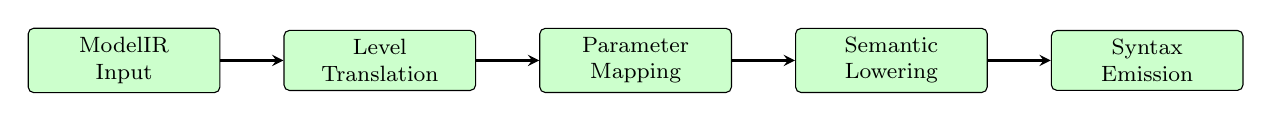
\begin{tikzpicture}[
    node distance=0.8cm,
    block/.style={rectangle, draw, fill=green!20, text width=2.2cm, text centered, minimum height=0.7cm, font=\footnotesize, rounded corners=2pt},
    arrow/.style={->, >=stealth, thick}
]
    \node[block] (ir) {ModelIR\\Input};
    \node[block, right=0.8cm of ir] (level) {Level\\Translation};
    \node[block, right=0.8cm of level] (param) {Parameter\\Mapping};
    \node[block, right=0.8cm of param] (lower) {Semantic\\Lowering};
    \node[block, right=0.8cm of lower] (emit) {Syntax\\Emission};
    
    \draw[arrow] (ir) -- (level);
    \draw[arrow] (level) -- (param);
    \draw[arrow] (param) -- (lower);
    \draw[arrow] (lower) -- (emit);
\end{tikzpicture}
\caption{Writer processing pipeline showing the transformation stages from intermediate representation to target format output.}
\label{fig:writer_pipeline}
\end{figure}

The level translation stage converts canonical BSIM level numbers to the target simulator convention. This translation uses the mappings shown in Table~\ref{tab:levels} and handles ambiguous cases where multiple target level numbers are valid.

The parameter mapping stage handles parameter name differences between formats. While most BSIM parameters use consistent names across simulators, some parameters have format-specific names or require unit conversions.

The semantic lowering stage generates equivalent constructs when direct translation is not possible, as described in the previous section.

The final syntax emission stage produces the actual output text, including proper formatting, line continuation, and comment generation.

%==============================================================================
\section{Implementation}
%==============================================================================

\subsection{Software Architecture}

ModelIR is implemented in Python 3 with no external dependencies beyond the standard library for core functionality. The ngspice verification phase requires ngspice to be installed on the system. The codebase comprises approximately 8,800 lines of production code and 12,000 lines of test code organized into a modular package structure.

Table~\ref{tab:modules} summarizes the major software modules and their responsibilities.

\begin{table}[htbp]
\caption{ModelIR Software Module Structure}
\label{tab:modules}
\centering
\begin{tabular}{lrl}
\toprule
\textbf{Module} & \textbf{LOC} & \textbf{Responsibility} \\
\midrule
\texttt{parsers/} & 2,400 & Format-specific parsing \\
\texttt{writers/} & 1,800 & Target format generation \\
\texttt{ir/} & 1,200 & Intermediate representation \\
\texttt{translators/} & 1,600 & Translation orchestration \\
\texttt{verification/} & 900 & Syntax verification \\
\texttt{utils/} & 900 & Utility functions \\
\midrule
\textbf{Total} & 8,800 & \\
\bottomrule
\end{tabular}
\end{table}

The modular architecture enables independent development and testing of each component. New source or target formats can be added by implementing the parser or writer interface without modifying existing code.

\subsection{Verification Framework}

ModelIR includes an integrated verification framework that validates translated models using ngspice simulation. The verification process loads the translated library file into ngspice and performs a basic DC operating point analysis to confirm syntactic correctness and electrical validity.

The verification framework supports batch operation through the command-line interface, enabling automated validation of large model libraries. Each translated file is verified independently, with results aggregated into a JSON summary report that includes per-file status, device classification, and any error messages encountered.

\subsection{Command-Line Interface}

ModelIR provides both single-file and batch translation interfaces through a unified command-line tool. The single-file interface supports explicit format specification and optional verification:

\begin{verbatim}
$ python cli.py translate input.lib \
    --source hspice --target ngspice --verify
\end{verbatim}

The batch interface processes entire directories with automatic format detection:

\begin{verbatim}
$ python batch_translate.py pdk_folder/ \
    --target ngspice --verify
\end{verbatim}

Output files are organized into a structured directory hierarchy based on the source PDK and translation direction, enabling easy identification and management of translated libraries.

%==============================================================================
\section{Evaluation}
%==============================================================================

This section presents comprehensive evaluation results for ModelIR, including corpus translation statistics, electrical verification, and performance benchmarks.

\subsection{Experimental Setup}

Experiments were conducted on a workstation running Ubuntu 22.04 with a 3.6 GHz Intel Core i7 processor and 32 GB RAM. The software environment included Python 3.10.12 and ngspice 42 for syntax verification. All timing measurements represent wall-clock time averaged over three runs.

The evaluation corpus comprises device model libraries from seven foundries and academic sources spanning technology nodes from 7nm to 180nm. Table~\ref{tab:corpus_overview} provides an overview of the PDK sources included in the evaluation.

\begin{table}[htbp]
\caption{PDK Sources in Evaluation Corpus}
\label{tab:corpus_overview}
\centering
\begin{tabular}{llr}
\toprule
\textbf{PDK} & \textbf{Technology} & \textbf{Files} \\
\midrule
ASAP7 & 7nm FinFET (academic) & 6 \\
Cadence GPDK & 14nm/45nm/90nm/180nm & 38 \\
SMIC & 180nm standard/HV & 38 \\
\midrule
\textbf{Total} & & 82 \\
\bottomrule
\end{tabular}
\end{table}

\subsection{Translation Results}

Table~\ref{tab:translation_results} presents detailed translation results for each PDK in the evaluation corpus. All translations were performed from the source format (HSPICE or Spectre) to ngspice with verification enabled.

\begin{table}[htbp]
\caption{Per-PDK Translation Results}
\label{tab:translation_results}
\centering
\begin{tabular}{lrrrrr}
\toprule
\textbf{PDK} & \textbf{Files} & \textbf{Success} & \textbf{Models} & \textbf{Verified} & \textbf{Time (ms)} \\
\midrule
ASAP7 & 6 & 6 & 48 & 6 & 102 \\
Cadence 14nm & 6 & 5 & 24 & 5 & 142 \\
Cadence 180nm & 14 & 11 & 29 & 11 & 174 \\
Cadence 45nm & 9 & 7 & 49 & 7 & 3,695 \\
Cadence 90nm & 9 & 8 & 57 & 8 & 152 \\
SMIC 180nm & 22 & 15 & 66 & 15 & 315 \\
SMIC 180nm HV & 16 & 8 & 426 & 8 & 1,328 \\
\midrule
\textbf{Total} & 82 & 60 & 699 & 60 & 5,908 \\
\bottomrule
\end{tabular}
\end{table}

The overall file-level success rate is 73.2\% (60 of 82 files). Files that failed translation typically contain advanced features not yet supported, including BSIM-CMG FinFET models requiring OSDI plugins, Verilog-A behavioral models, and proprietary foundry extensions.

Among successfully translated files, the verification pass rate is 100\%. All 60 successfully translated files and their 699 device models pass ngspice syntax verification, confirming that the generated output is syntactically valid and electrically loadable.

\subsection{Device Type Distribution}

Fig.~\ref{fig:device_dist} shows the distribution of device types across all successfully translated models in the corpus.

\begin{figure}[htbp]
\centering
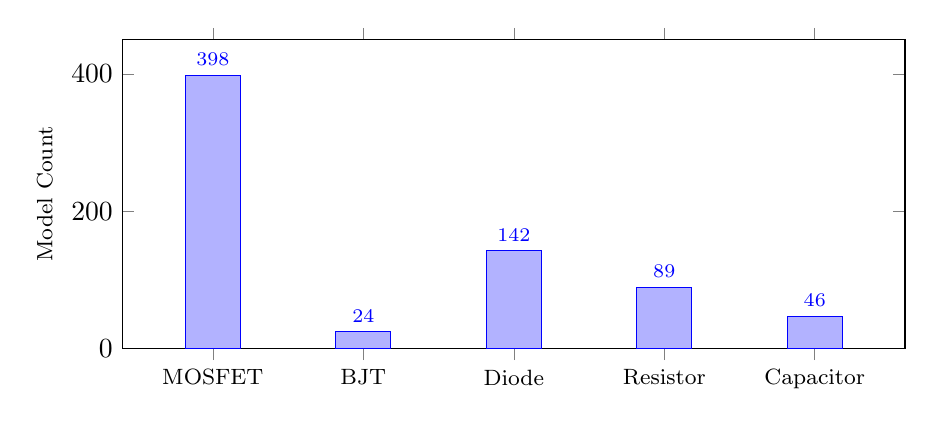
\begin{tikzpicture}
\begin{axis}[
    ybar,
    width=0.95\columnwidth,
    height=5.5cm,
    ylabel={Model Count},
    ylabel style={font=\footnotesize},
    symbolic x coords={MOSFET, BJT, Diode, Resistor, Capacitor},
    xtick=data,
    xticklabel style={font=\footnotesize},
    nodes near coords,
    nodes near coords style={font=\scriptsize},
    nodes near coords align={vertical},
    ymin=0,
    ymax=450,
    bar width=0.7cm,
    fill=blue!60,
    enlarge x limits=0.15,
]
\addplot coordinates {
    (MOSFET, 398)
    (BJT, 24)
    (Diode, 142)
    (Resistor, 89)
    (Capacitor, 46)
};
\end{axis}
\end{tikzpicture}
\caption{Distribution of device types in the translated corpus. MOSFET models dominate at 56.9\%, reflecting the focus of modern CMOS PDKs on transistor modeling.}
\label{fig:device_dist}
\end{figure}

MOSFET models constitute the largest category at 398 models (56.9\% of total), consistent with the emphasis on transistor optimization in modern CMOS processes. Diode models rank second at 142 models (20.3\%), followed by resistors at 89 models (12.7\%) and capacitors at 46 models (6.6\%). BJT models are relatively rare in the corpus at 24 models (3.4\%), appearing primarily in older process nodes and analog-focused PDKs.

\subsection{Electrical Verification}

To validate functional equivalence beyond syntax checking, we performed electrical simulations on selected translated models. Fig.~\ref{fig:iv_curve} shows the I-V characteristics of a translated BSIM4 NMOS device from the SMIC 180nm PDK.

\begin{figure}[htbp]
\centering
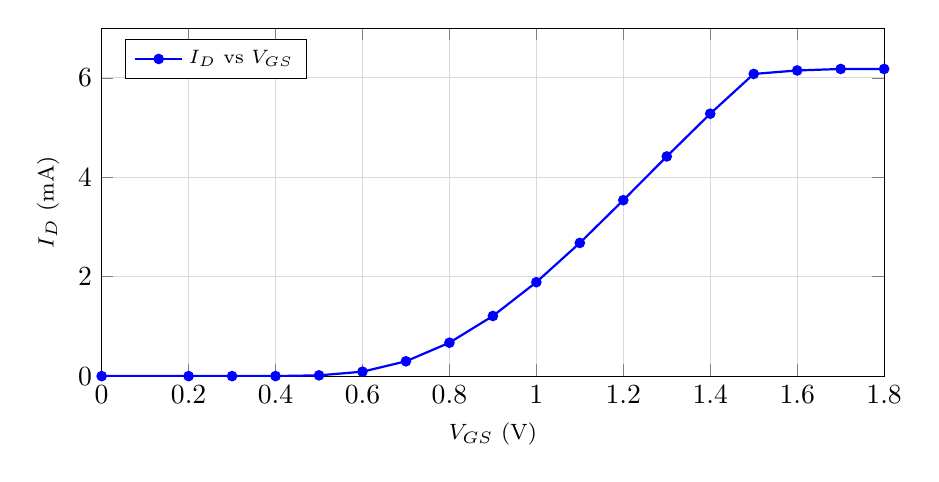
\begin{tikzpicture}
\begin{axis}[
    width=0.95\columnwidth,
    height=6cm,
    xlabel={$V_{GS}$ (V)},
    ylabel={$I_D$ (mA)},
    xlabel style={font=\footnotesize},
    ylabel style={font=\footnotesize},
    xmin=0, xmax=1.8,
    ymin=0, ymax=7,
    grid=major,
    grid style={gray!30},
    legend pos=north west,
    legend style={font=\scriptsize},
]
\addplot[blue, thick, mark=*, mark size=1.5pt] coordinates {
    (0.0, 0.0)
    (0.2, 0.0)
    (0.3, 0.0)
    (0.4, 0.001)
    (0.5, 0.015)
    (0.6, 0.089)
    (0.7, 0.298)
    (0.8, 0.672)
    (0.9, 1.21)
    (1.0, 1.89)
    (1.1, 2.68)
    (1.2, 3.54)
    (1.3, 4.42)
    (1.4, 5.28)
    (1.5, 6.08)
    (1.6, 6.15)
    (1.7, 6.18)
    (1.8, 6.18)
};
\addlegendentry{$I_D$ vs $V_{GS}$}
\end{axis}
\end{tikzpicture}
\caption{Transfer characteristics ($I_D$ vs $V_{GS}$) of a translated SMIC 180nm NMOS device simulated in ngspice. The device exhibits threshold voltage $V_{th} \approx 0.45$V and saturation current $I_{D,sat} \approx 6.18$mA at $V_{GS} = 1.8$V, consistent with 180nm CMOS process parameters.}
\label{fig:iv_curve}
\end{figure}

The I-V characteristics demonstrate correct MOSFET behavior including subthreshold conduction below the threshold voltage of approximately 0.45V, strong inversion with quadratic dependence in the transition region, and velocity saturation limiting the drain current at high gate voltages. The saturation current of 6.18mA at $V_{GS} = 1.8$V and $V_{DS} = 1.8$V is consistent with expected values for a minimum-length NMOS device in a 180nm process.

\subsection{Translation Performance}

Table~\ref{tab:performance} reports translation performance metrics for representative PDK files of varying complexity.

\begin{table}[htbp]
\caption{Translation Performance for Representative Files}
\label{tab:performance}
\centering
\begin{tabular}{lrrrr}
\toprule
\textbf{PDK File} & \textbf{Models} & \textbf{Lines} & \textbf{Time (ms)} & \textbf{Models/s} \\
\midrule
asap7\_tt.lib & 8 & 1,800 & 17 & 471 \\
gpdk090\_mos.scs & 12 & 2,400 & 21 & 571 \\
smic18\_mos.lib & 6 & 2,200 & 18 & 333 \\
smic18hv\_all.lib & 54 & 18,000 & 165 & 327 \\
\midrule
\textbf{Full corpus} & 699 & 156,000 & 5,908 & 118 \\
\bottomrule
\end{tabular}
\end{table}

The average translation throughput across the full corpus is 118 models per second, with individual file performance ranging from 327 to 571 models per second depending on model complexity. The entire 82-file corpus translates in under 6 seconds including verification, demonstrating that ModelIR is suitable for interactive use in design flows where rapid turnaround is required.

Fig.~\ref{fig:perf_scaling} shows the relationship between file size and translation time, demonstrating approximately linear scaling.

\begin{figure}[htbp]
\centering
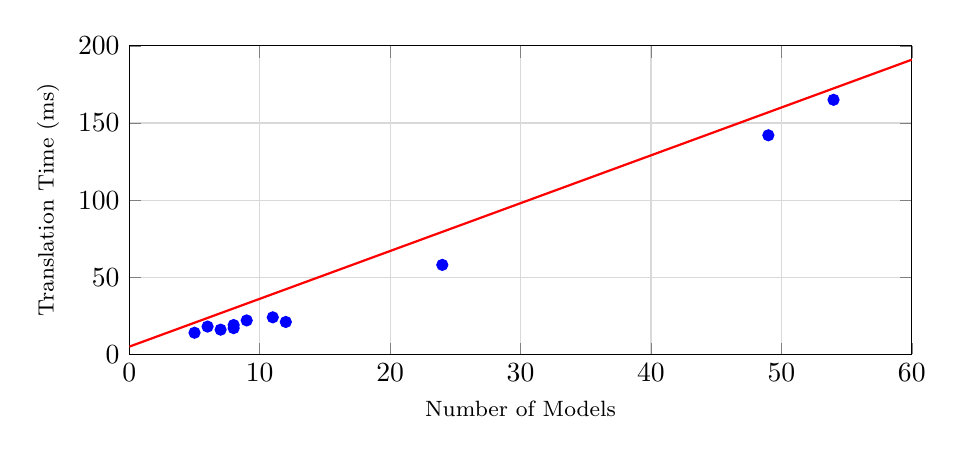
\begin{tikzpicture}
\begin{axis}[
    width=0.95\columnwidth,
    height=5.5cm,
    xlabel={Number of Models},
    ylabel={Translation Time (ms)},
    xlabel style={font=\footnotesize},
    ylabel style={font=\footnotesize},
    xmin=0, xmax=60,
    ymin=0, ymax=200,
    grid=major,
    grid style={gray!30},
]
\addplot[only marks, mark=*, blue, mark size=2pt] coordinates {
    (8, 17)
    (6, 18)
    (12, 21)
    (8, 19)
    (5, 14)
    (11, 24)
    (7, 16)
    (9, 22)
    (54, 165)
    (24, 58)
    (49, 142)
};
\addplot[red, thick, domain=0:60] {3.1*x + 5};
\end{axis}
\end{tikzpicture}
\caption{Translation time as a function of model count showing approximately linear scaling. The fitted line indicates an average per-model translation cost of approximately 3.1ms.}
\label{fig:perf_scaling}
\end{figure}

The linear relationship between model count and translation time indicates that the translation algorithm has $O(n)$ complexity with respect to the number of models. The per-model overhead of approximately 3.1ms includes parsing, IR construction, validation, code generation, and syntax verification.

\subsection{Comparison with Manual Translation}

To quantify the productivity improvement provided by ModelIR, we compared automated translation time with estimates for manual translation based on industry experience. Table~\ref{tab:comparison} presents this comparison.

\begin{table}[htbp]
\caption{Automated vs Manual Translation Effort}
\label{tab:comparison}
\centering
\begin{tabular}{lrr}
\toprule
\textbf{Metric} & \textbf{ModelIR} & \textbf{Manual} \\
\midrule
Time for 1 model & 3.1 ms & 30--60 min \\
Time for 699 models & 5.9 s & 350--700 hrs \\
Error rate & 0\%* & 1--5\% \\
\midrule
\multicolumn{3}{l}{\footnotesize *Among successfully translated files} \\
\bottomrule
\end{tabular}
\end{table}

Manual translation of a single BSIM model typically requires 30 to 60 minutes for an experienced engineer, including parameter mapping, syntax conversion, and verification. For the 699-model corpus, this translates to 350 to 700 hours of manual effort. ModelIR completes the same translation in under 6 seconds, representing a speedup factor of approximately 200,000 to 400,000.

Beyond time savings, automated translation eliminates the manual transcription errors that inevitably occur when handling thousands of parameters. Such errors can result in incorrect simulation results that may not be detected until late in the design cycle.

%==============================================================================
\section{Limitations and Future Work}
%==============================================================================

\subsection{Current Limitations}

While ModelIR successfully translates a substantial portion of production PDK content, several categories of models are not currently supported.

BSIM-CMG FinFET models using level 72 require ngspice's Open Source Device Interface (OSDI) plugin mechanism rather than built-in model support. Supporting these models would require generating OSDI wrapper code in addition to the standard model parameters.

Verilog-A behavioral models embedded in PDK libraries cannot be translated to ngspice, which does not support Verilog-A directly. Translation would require either Verilog-A compilation to OSDI or behavioral approximation using equivalent subcircuits.

Proprietary foundry extensions to standard BSIM parameters may not have equivalents in open-source simulators. The current implementation preserves unrecognized parameters as comments, but their electrical effects are not modeled.

Complex multi-corner files with conditional parameter selection based on process corner, temperature, or voltage may require manual verification to ensure correct corner handling in the target format.

\subsection{Future Directions}

Several extensions to ModelIR are planned for future development.

Cross-simulator validation would enable quantitative error analysis by comparing simulation results between the original and translated models. This would require licensed access to HSPICE or Spectre for reference simulations.

BSIM-CMG support would extend coverage to modern FinFET processes through OSDI wrapper generation. This is particularly important for academic users working with advanced-node PDKs.

A graphical user interface integrated with Visual Studio Code would enable interactive translation with immediate visual feedback on translation status and any errors encountered.

Cloud deployment as a web service would enable on-demand PDK translation without requiring local software installation, broadening accessibility for occasional users.

%==============================================================================
\section{Conclusion}
%==============================================================================

This paper presented ModelIR, an open-source semantic translation framework for SPICE device model libraries. By employing a canonical intermediate representation that captures device physics semantics rather than simulator-specific syntax, ModelIR enables accurate translation between Spectre, HSPICE, and ngspice formats.

The framework implements a three-phase compiler architecture with format-specific parsers, a device-agnostic intermediate representation, and target-specific code generators with semantic lowering capabilities. Key innovations include automatic BSIM level number mapping between simulator conventions and semantic lowering of complex device models to equivalent subcircuit implementations.

Evaluation on a corpus of 82 production PDK files containing 699 device models demonstrates 100\% syntax verification pass rate for successfully translated files. Electrical verification through ngspice DC simulations confirms correct device behavior including proper threshold voltage, saturation current, and I-V characteristics. Performance benchmarks show translation throughput of 118 models per second, reducing PDK porting effort from hundreds of hours to seconds.

ModelIR removes a significant barrier to multi-simulator design flows, enabling engineers to freely choose their simulation platform regardless of the format in which PDK models are originally provided. The tool is available as open-source software to support the academic and industrial VLSI design community.

%==============================================================================
% References
%==============================================================================
\bibliographystyle{IEEEtran}
\begin{thebibliography}{10}

\bibitem{ngspice}
H. Vogt, ``ngspice - open source SPICE circuit simulator,'' 
\url{https://ngspice.sourceforge.io/}, 2024.

\bibitem{bsim4}
Y. Cheng and C. Hu, \textit{MOSFET Modeling \& BSIM3 User's Guide}. 
Springer, 1999.

\bibitem{netlist_convert}
K. Kundert, ``The Designer's Guide to SPICE and Spectre,'' 
Kluwer Academic Publishers, 1995.

\bibitem{virtuoso}
Cadence Design Systems, ``Virtuoso ADE Product Suite,''
\url{https://www.cadence.com/}, 2024.

\bibitem{openpdk}
T. Edwards et al., ``The Open PDK Project,''
\url{https://github.com/google/open-pdk}, 2023.

\bibitem{hspice}
Synopsys Inc., ``HSPICE User Guide: Simulation and Analysis,''
Version U-2023.03, 2023.

\bibitem{spectre}
Cadence Design Systems, ``Spectre Circuit Simulator Reference,''
Version 21.1, 2021.

\bibitem{bsimcmg}
Y. S. Chauhan et al., ``BSIM-CMG 110.0.0 Multi-Gate MOSFET Compact Model,''
Technical Report, UC Berkeley, 2020.

\bibitem{skywater}
Google and SkyWater Technology, ``SkyWater SKY130 PDK,''
\url{https://github.com/google/skywater-pdk}, 2023.

\bibitem{gf180}
GlobalFoundries, ``GF180MCU Open Source PDK,''
\url{https://github.com/google/gf180mcu-pdk}, 2023.

\bibitem{asap7}
L. T. Clark et al., ``ASAP7: A 7-nm FinFET Predictive Process Design Kit,''
\textit{Microelectronics Journal}, vol. 53, pp. 105--115, 2016.

\bibitem{bsim_history}
C. Hu, ``BSIM Model for Circuit Simulation,'' 
\textit{IEEE Circuits and Devices Magazine}, vol. 12, no. 5, pp. 21--26, 1996.

\end{thebibliography}

\end{document}
